%!TEX root = ../NCVC.tex

\section{基本編}

\subsection{CADでの作図}
 まずは基本的な加工を行うための基本的な作図方法を解説します.

\begin{minipage}[t]{0.3\textwidth}
\vspace*{1zh}
 図\ref{fig:sample1.jww}のような図形を書きましょう.
切削対象(ワーク)を示す矩形と,その矩形左下に円を1つ.
「NCVC」という文字は,線をつなぎ合わせたデータです.
\end{minipage}
\begin{minipage}[t]{0.7\textwidth}
\begin{figure}[H]
\centering
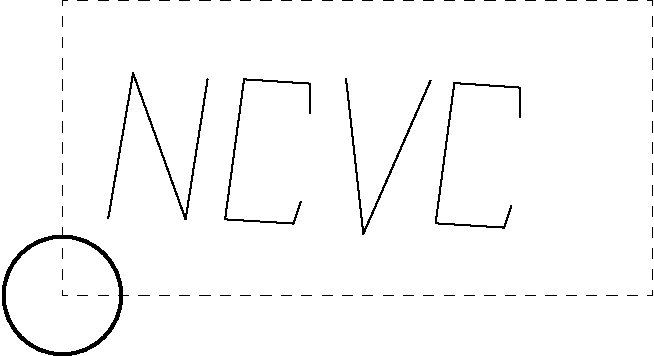
\includegraphics[scale=0.8]{No1/fig/sample1.pdf}
\caption{サンプル図形}
\label{fig:sample1.jww}
\end{figure}
\end{minipage}

\vspace*{1zh}
 NCVCはCADでの作図情報を全て読み込むのではなく,
特定のレイヤ情報を元に作図データを読み込みます.
CADでの作図において必要とされる補助線や寸法線等が加工データには必要なく,
これらを選別するための仕様です.

 その選別方法は『必要なレイヤに名前を付ける』こと.
図\ref{fig:sampleLayer.png} は図\ref{fig:sample1.jww}のレイヤ情報ですが,
0番レイヤに「ORIGIN」という名前,
1番レイヤに「CAM\_LINE」という名前を付けています.
それぞれ機械原点と切削軌跡を示し,この2つのレイヤは必須です
\footnote{実は機械原点レイヤは必須ではありません.詳細は「穴加工」の節で解説しています.}.
機械原点レイヤには工作機械のXY原点を示す円を1つだけ作図.
大きさは任意ですが,円の中心がXYの原点となります.
切削軌跡 CAM\_LINE レイヤには刃物のパス,
すなわち削りたい図形を書きます.
他,ワーク矩形を示す補助線等は別のレイヤに書きます.
なお,全てのデータにおいて線種,線色は関係ありません.

\begin{figure}[H]
\centering
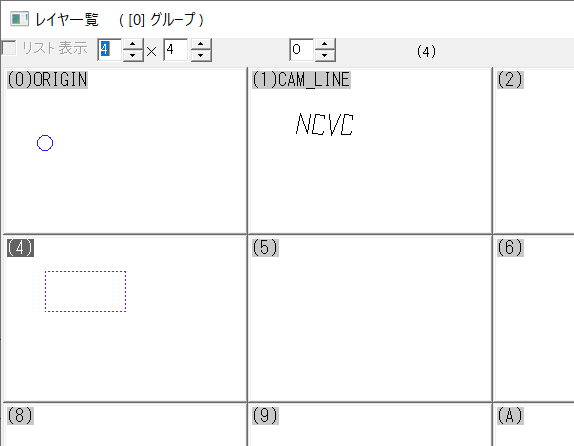
\includegraphics{No1/fig/sampleLayer.png}
\caption{レイヤ一覧}
\label{fig:sampleLayer.png}
\end{figure}

 レイヤに名前を付ける方法は,それぞれのCAD操作に準拠して下さい.

 作図が終わればCADデータをDXF形式で保存します
\footnote{
    Jw\_cadの場合,DXF形式で保存する必要はありません.NCVCはJWW形式を直接読み込むことが可能です.
    詳細は「パワーユーザ編」の「アドイン作成のすすめ」を参照して下さい.
}.
NCVCにCADデータを読み込ませるためDXF形式で保存する必要がありますが,
多くの場合,DXF形式で保存するとそのCAD独自のデータが失われるため,
使用しているCAD独自の形式でも保存しておきましょう.

\subsection{CADデータの読み込み}
